\subsection{复余切丛与量子化}\label{ccb}

现在回到实辛流形 $M=T^*N$，问 $Y=T^*W$（$W$ 为 $M$ 的复化）的 $A$-模型如何用来研究 $M$ 的量子化。

我们将利用另一个 $(B,A,A)$ 型拉格朗日膜 $\cF$。在进入细节前，先说明策略（第 \ref{smooth} 节已简述）。我们将描述相当自然的元素 $\alpha\in\Hom(\B_\cc,\cF)$ 与 $\beta\in\Hom(\cF,\B)$，其中 $\B_\cc$ 仍为典范余各向同性 $A$-膜，$\B$ 为支撑在 $M$ 上的秩 1 拉格朗日 $A$-膜。一旦定义了 $\alpha$ 与 $\beta$，就容易用三元组 $\cF,\alpha,\beta$ 定义 $\H'=\Hom(\B_\cc,\B)$ 中的元素 $\psi'$，而 $\H'$ 是 Hilbert 空间 $\H=\Hom(\B,\B_\cc)$ 的对偶。（第 \ref{hermitian} 节定义的自然反线性映射 $\Theta_\tau$ 给出 $\H$ 与 $\H'$ 的同构，但在不引用它时，我们区分 $\H$ 与 $\H'$。）其实，对我们将要选取的 $\cF$，$\psi'$ 将是分布波函数。这与第 \ref{smooth} 节的讨论一致，因为 $\cF$ 没有紧支撑。

代数上，把 $\alpha\in\Hom(\B_\cc,\cF)$ 与 $\beta\in\Hom(\cF,\B)$ 复合，得 $\psi'=\beta\circ\alpha\in\H'=\Hom(\B_\cc,\B)$。用图来说，就是考虑图 \ref{strip} 中的条带，$\B_\cc$ 在左、$\cF$ 在上、$\B$ 在右，角上为 $\alpha,\beta$。受此类图启发，我们把 $\alpha,\beta$ 这样的对象称为\textbf{角}。\footnote{在二维中，把这些对象称为“角”似乎缺乏动机，因为这些角可通过共形映射拉直。这个术语的动机来自二维以上的类似构造：在那里这种表示两种不同边界条件衔接的角不能被共形拉直。关于某些四维超对称理论中此类衔接的系统研究见 \cite{GR}。这样的四维构造可通过黎曼面上的紧化约化到二维，这与几何 Langlands 有关。}条带上的路径积分自然产生向量 $\psi'\in\H'=\Hom(\B_\cc,\B)$。确实，若提供态 $\psi\in\Hom(\B,\B_\cc)$ 作为条带底部的边界条件，则条带上的路径积分只产生一个数。与图 \ref{strip} 类似但 $\F$ 在底部的图产生 $\H$ 中的向量，这已在第 \ref{smooth} 节解释。

\begin{figure}[htbp]
 \centering
 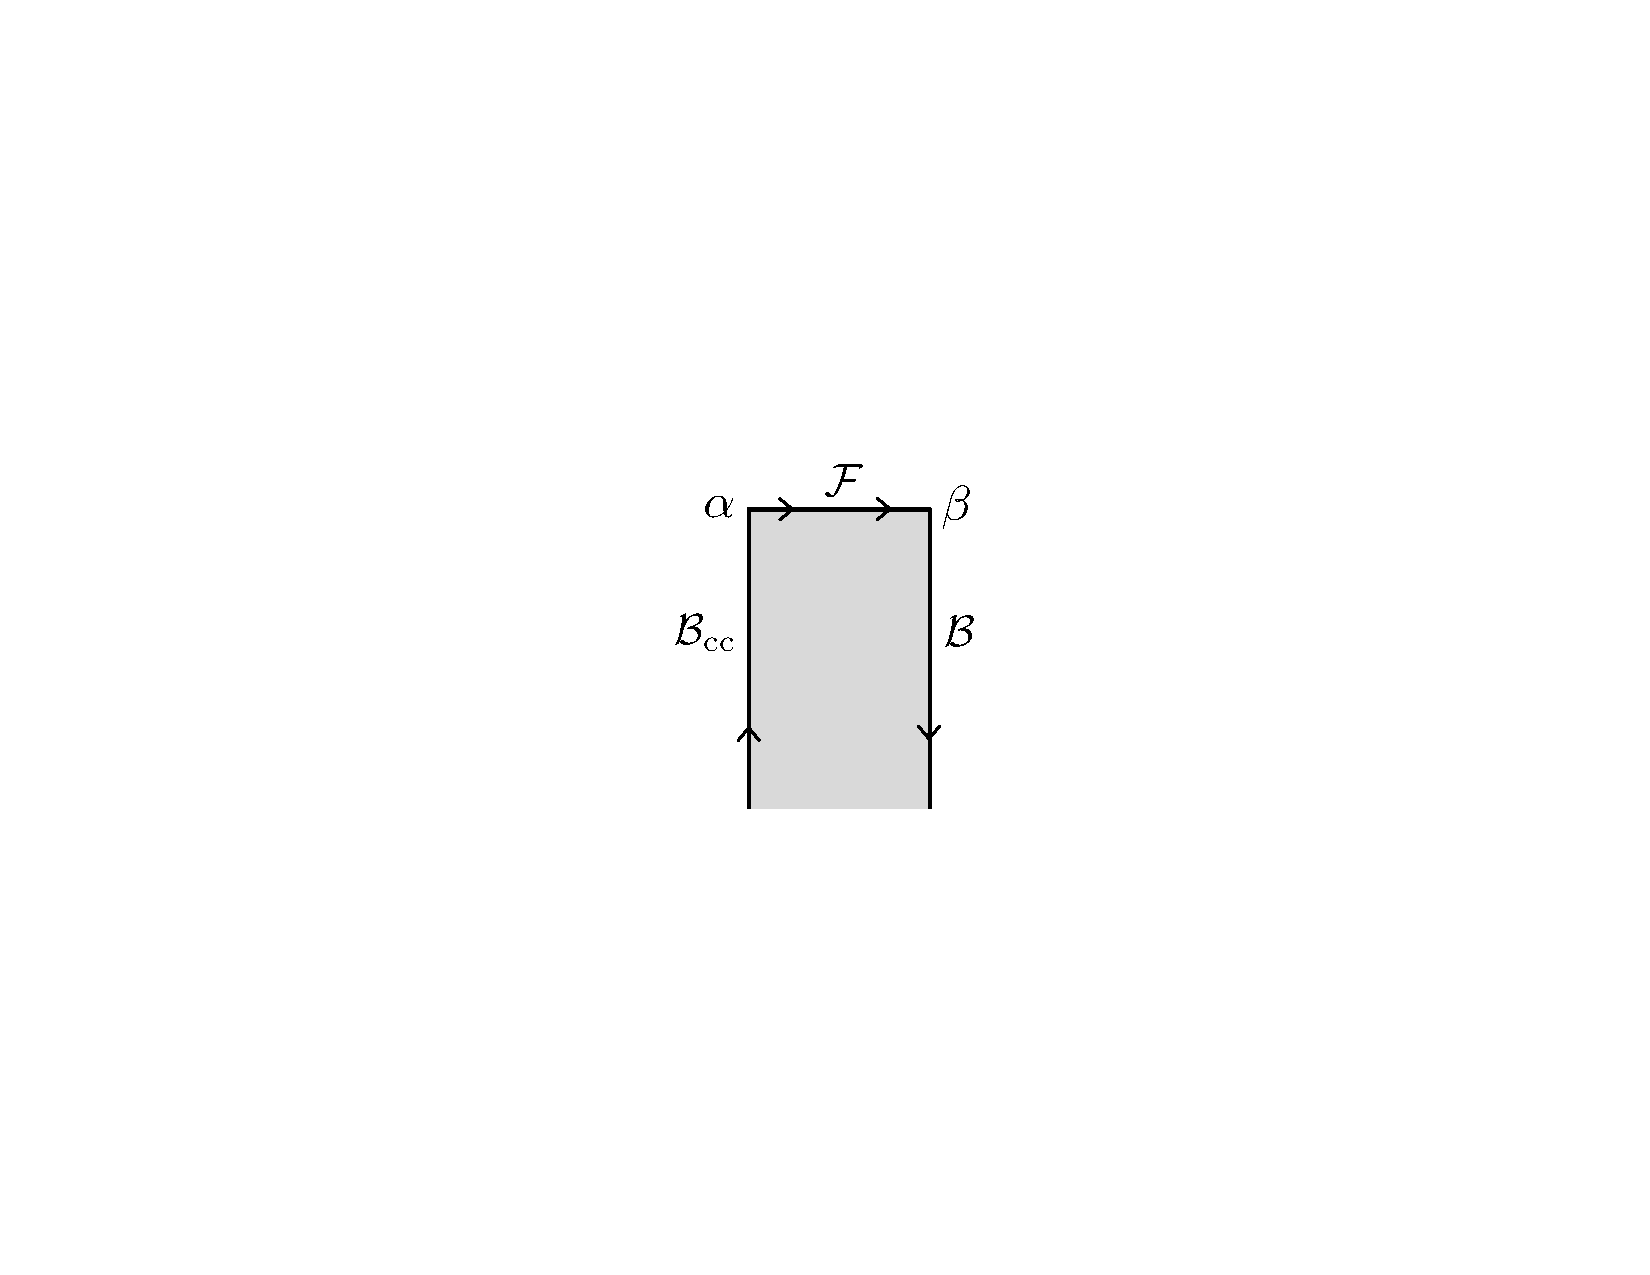
\includegraphics[width=0.36\textwidth]{figures/2_Strip.pdf}
 \caption{\small 条带，$\B_\cc$ 在左、$\F$ 在上、$\B$ 在右，角上为适当的 $\alpha,\beta$。按图 \ref{explained}(a) 的约定，$\alpha$ 表示 $\Hom(\B_\cc,\F)$ 的元素，$\beta$ 表示 $\Hom(\F,\B)$ 的元素；它们的合成是 $\H'=\Hom(\B_\cc,\B)$ 的元素。图中该元素从条带顶部（它在此产生）向下传播。}
 \label{strip}
\end{figure}

对 $\cF$，取支撑在余切丛 $T^*W$ 的纤维 $F$ 上的膜，$F$ 是包含某点 $w\in W$ 的纤维。最终将专门取 $w\in N$，但暂时允许任意 $w$。把 $w$ 邻域中 $W$ 的局部坐标记作 $q^i$，把余切丛纤维上的共轭函数记作 $p_i$。

由于 $F\cong\C^n$ 有唯一 spin 结构，$\cF$ 的 $\CP$ 丛就是平坦线丛；又因 $F$ 单连通，这个平坦线丛平凡。$F$ 在余切丛伸缩下不变（虽非逐点不变），故 $\cF$ 也在此伸缩下不变。于是如第 \ref{lagbr} 节，$\Hom(\B_\cc,\cF)$ 可在 $\hbar\to0$ 极限下计算。仍由附录 \ref{details}，结果为 $\Hom(\B_\cc,\cF)=H^0(F,K_F^{1/2})$，这里用了 $F\cong\C^n$ 时高阶上同调消失。此外 $K_F^{1/2}$ 平凡，故 $H^0(F,K_F^{1/2})$ 等同于 $F$ 上的全纯函数空间。由于不允许在无穷远指数增长的波函数，$H^0(F,K_F^{1/2})$ 可等同于参数化 $F$ 的坐标 $p_i$ 的多项式函数空间。我们要取\footnote{记号上不区分 $\alpha\in H^0(F,K_F^{1/2})$ 与 $\Hom(\B_\cc,\F)$ 中对应的元素；稍后对 $\beta$ 也类似。}处处非零的 $\alpha\in H^0(F,K_F^{1/2})$，即它给出平凡线丛 $K_F^{1/2}$ 的平凡化。这样的 $\alpha$ 一旦在一点取定便唯一确定，该点取为 $F\cap W$ 的唯一交点 $w$。我们取\footnote{\label{funnysign}下述描述不确定 $\alpha$ 的符号。此符号的可能意义见脚注 \ref{maybe}。}$\alpha|_w=(\d p_1\d p_2\cdots\d p_n)^{1/2}$，意思是 $K_F^{1/2}$ 中在同构 $(K_F^{1/2})^2=K_F$ 下映到 $\d p_1\d p_2\cdots\d p_n$ 的向量。简记为 $\alpha=(\d\vec p)^{1/2}$。

还需定义元素 $\beta\in\Hom(\cF,\B)$。由于 $\B$ 与 $\cF$ 都是拉格朗日膜（分别支撑在 $M$ 与 $F$ 上），这是 $A$-模型中的标准构件。$\Hom(\cF,\B)$ 的首阶近似是交集 $M\cap F$ 上取值于 $\CP$ 丛适当张量积的上同调。在投影 $T^*W\to W$ 下，$M$ 投到 $N$，$F$ 投到 $w$，故除非 $w\in N$，交集 $M\cap F$ 为空。所以若 $w\notin N$，则 $\Hom(\cF,\B)=0$。因此限制到 $w\in N$。此时 $M\cap F$ 就是实余切丛 $T^*N$ 在 $w$ 处的纤维，即 $\R^n$ 的拷贝，记作 $F_M$。由于 $\cF$ 的 $\CP$ 丛平凡，相关的 $\CP$ 丛张量积就是 $\L$，即 $\B$ 的 $\CP$ 丛。于是 $\Hom(\cF,\B)$ 的首阶近似是 $\oplus_{r=0}^nH_{\mathrm{dR}}^r(F_M,\L)$，这里所论上同调是 $F_M$ 上取值于平坦线丛 $\L|_{F_M}$ 的 de Rham 上同调。由于 $F_M\cong\R^n$，此上同调除 $r=0$ 外消失。一般地，对拉格朗日 $A$-膜 $\B,\cF$，交集上同调只是 $\Hom(\cF,\B)$ 的初步近似；但此处上同调除一个 $r$ 值外消失，故这就是完整答案：$\Hom(\cF,\B)=H_{\mathrm{dR}}^0(F_M,\L)$。这个上同调群由 $\L\to F_M$ 的协变常截面组成。故 $\beta$ 可取 $\L$ 在 $F_M$ 上的任一协变常截面。方便的是把协变常截面与其在点 $w\in F_M$ 处的值等同，于是可把 $\beta$ 看作 $\L_w$（$\L$ 在 $w$ 处的纤维）中的向量。

对任意 $w\in N$ 及如上选取的 $\alpha,\beta$，此构造确定态 $\psi'(w;\alpha,\beta)\in\H'$。为理解这些态的含义，我们来计算 $\psi'(w;\alpha,\beta)$ 与另一态 $\psi'(w';\alpha',\beta')$ 的内积；后者类似地由支撑在余切丛于另一点 $w'\in N$ 的纤维 $F'$ 上的膜 $\cF'$ 及如上定义的 $\alpha',\beta'$ 给出。为定义此内积，使用第 \ref{hermitian} 节引入的 $\H'$ 的 Hilbert 空间结构。定义的主要步骤是对其中一个态作用 $\Theta_\tau=\Theta\tau$，其中 $\Theta$ 是 $\CPT$，$\tau$ 是保持 $M$ 不动的 $Y$ 的反全纯对合。例如把 $\Theta_\tau$ 作用在 $\psi'(w';\alpha',\beta')$ 上。由于 $\tau$ 保持 $M$ 不动，它把 $w'\in N\subset M$ 映到自身。因此它把 $T^*W$ 在 $w'$ 处的纤维映到自身（非逐点）。结果是 $\Theta_\tau$ 只把膜 $\cF'$ 映到自身，同时反转弦的定向并对 $\alpha',\beta'$ 取复共轭。考虑到这一点，Hilbert 空间内积 $\langle\psi'(w';\alpha',\beta'),\psi'(w;\alpha,\beta)\rangle$ 可由图 \ref{rectangle} 所示矩形上的路径积分计算。该矩形由以下方式构造：取图 \ref{strip} 的条带与把 $\cF$ 换成 $\cF'$ 的类似条带，在把第二条带上下翻转以计入 $\Theta_\tau$ 的作用后粘合起来。（第二条带上下翻转时，角上的波函数 $\alpha',\beta'$ 取复共轭，以计入 $\Theta_\tau$ 的作用。）

\begin{figure}[htbp]
 \centering
 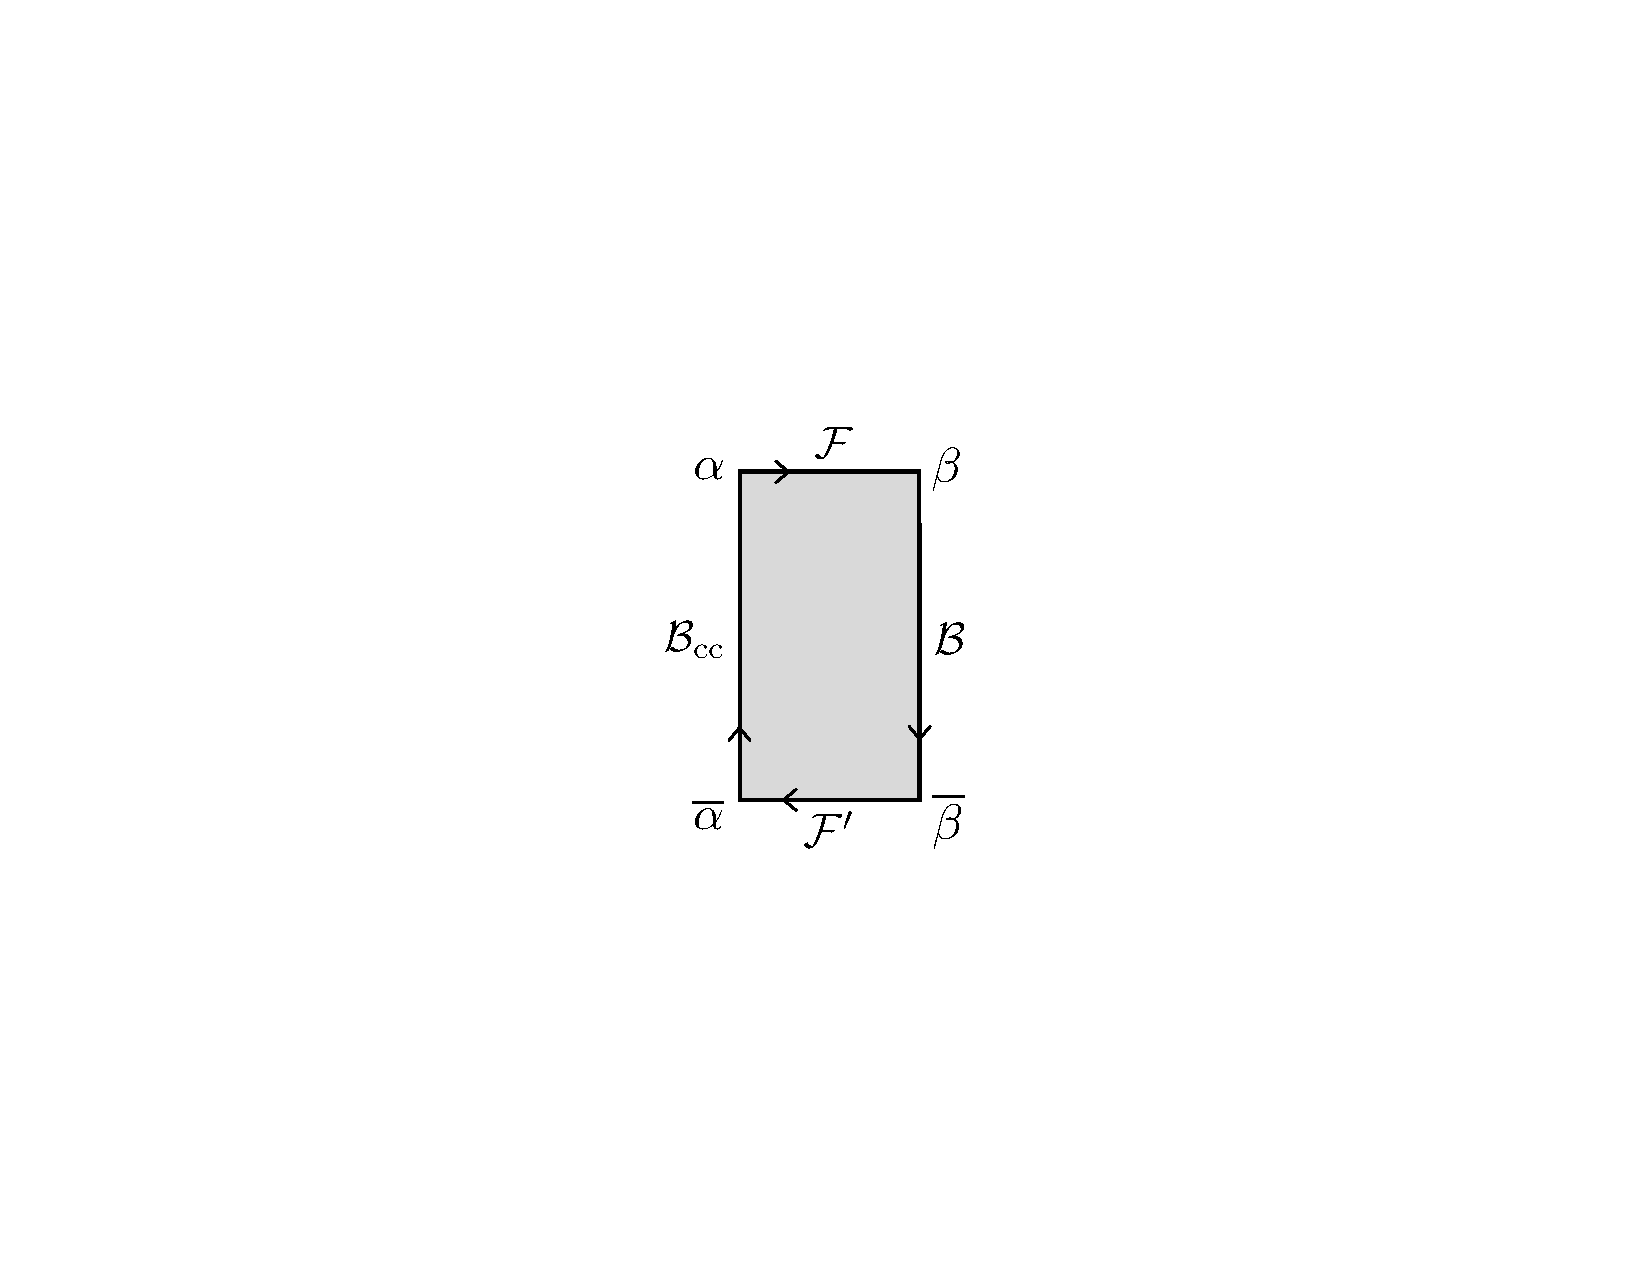
\includegraphics[width=0.36\textwidth]{figures/3.pdf}
 \caption{\small 由 $\F$ 与 $\F'$ 产生的态之间的内积，可通过此矩形上的路径积分计算。}
 \label{rectangle}
\end{figure}

我们断言：若 $w\ne w'$，则 $\langle\psi'(w';\alpha',\beta'),\psi'(w;\alpha,\beta)\rangle=0$。为证明这一点，利用 $A$-模型的二维拓扑不变性。我们通过讨论 Hilbert 空间 $\H=\Hom(\B_\cc,\B)$ 中从矩形底部传播到顶部的态来引入矩形；但也可等价地把矩形看作描述从左到右的传播。如图 \ref{secondone}(a) 所示，若利用拓扑不变性把矩形从左向右拉长，这第二种看法就很自然。图中从左向右传播的态是 $\Hom(\cF',\cF)$ 的元素。由于 $\cF$ 与 $\cF'$ 分别是支撑在 $F$ 与 $F'$ 上的拉格朗日 $A$-膜，计算 $\Hom(\cF,\cF')$ 的起点是交集 $F\cap F'$ 的上同调。但若 $w\ne w'$，则 $F\cap F'=\varnothing$，故 $\Hom(\cF,\cF')=0$，从而 $\langle\psi'(w';\alpha',\beta'),\psi'(w;\alpha,\beta)\rangle=0$。

\begin{figure}[htbp]
 \centering
 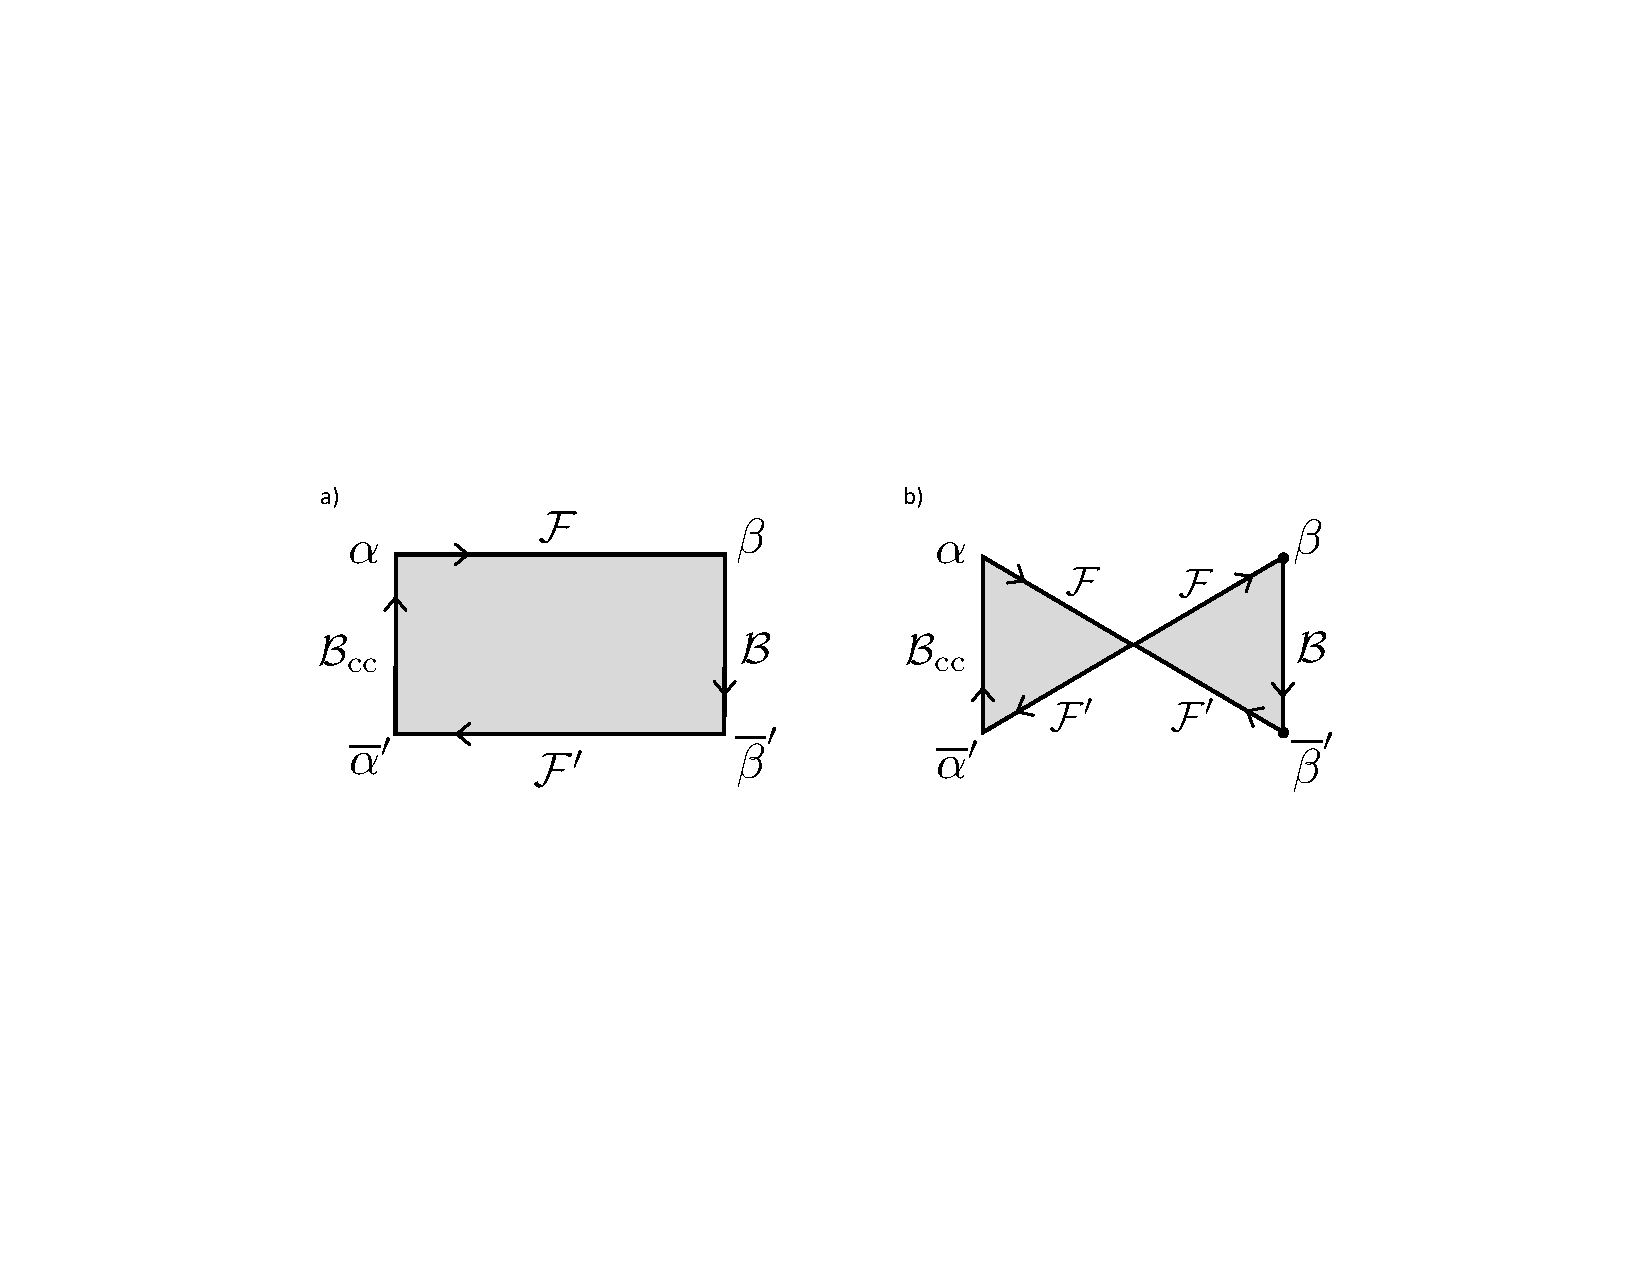
\includegraphics[width=0.72\textwidth]{figures/4.pdf}
 \caption{\small (a) 可把图 \ref{rectangle} 的矩形看作描述 $\Hom(\B,\B_\cc)$ 的元素从图底部到顶部的传播，或描述 $\Hom(\F',\F)$ 的元素从左到右的传播。把图形从左向右拉长会提示第二种解释。由于二维拓扑不变性，矩形的度量结构无关紧要。(b) 在某个极限下，矩形退化为两个在顶点粘合的三角形。穿过顶点的是 $\Hom(\F',\F)$ 中的一个态。可通过按 $\Hom(\F',\F)$ 的一组基态求和、并对每个基态计算两个三角形之积来求矩形的值。}
 \label{secondone}
\end{figure}

有时我们会在 $\Hom(\cF,\cF')$ 不为零的情形遇到类似矩形。为将来参考，注意这种矩形上的拓扑场论路径积分可这样计算：让矩形退化为在顶点粘合的一对三角形，如图 \ref{secondone}(b) 所示。左三角形涉及 $\B_\cc$ 与两个 $(B,A,A)$ 型膜；我们称这样的三角形为\textbf{全纯三角形}。右三角形涉及三个拉格朗日膜 $\cF,\cF',\B$；我们称之为\textbf{拉格朗日三角形}。

由于 $w\ne w'$ 时 $\langle\psi'(w';\alpha',\beta'),\psi'(w;\alpha,\beta)\rangle=0$，自然应把 $\psi'(w;\alpha,\beta)$ 视为支撑在点 $w\in N$ 处的 delta 函数态。若是如此，则预期 $\langle\psi'(w';\alpha',\beta'),\psi'(w;\alpha,\beta)\rangle$ 正比于 $\delta(w,w')$。遗憾的是，我们尚未找到通过研究矩形上路径积分来显式展示这个 delta 函数的方便办法。作为替代，我们将用其它方式探究 $\psi'(w;\alpha,\beta)$ 作为 delta 函数的解释。

回忆几何量子化的通常配方：把 $M=T^*N$ 作为余切丛量子化所得的 Hilbert 空间 $\H$，是 $N$ 上取值于预量子线丛 $\frL$ 的半密度空间。这意味着 $\H$ 的对偶空间是 $N$ 上取值于 $\frL$ 的对偶的半密度空间。在膜构造中，$\frL=\L^{-1}$，即 $\B$ 的 $\CP$ 丛之逆。

若 $f,g$ 分别是 $N$ 上取值于 $\L$ 与 $\L^{-1}$ 的半密度，则有自然双线性（非 Hermite）配对 $(f,g)=\int_Nfg$。故按几何量子化，$\H$ 的对偶应由 $N$ 上取值于 $\L$ 的半密度组成。来看能否把 $\psi'(w;\alpha,\beta)$ 解释为 $N$ 上支撑在 $w$ 处、取值于 $\L_w$ 的半密度。首先注意 $\psi'(w;\alpha,\beta)$ 正比于 $\beta$，而 $\beta$ 取值于 $\L_w$。还需理解如何把 $\psi'(w;\alpha,\beta)$ 解释为 $N$ 上支撑在 $w$ 处的半密度。

$N$ 上的密度丛是平凡实线丛，记作 $\K_N$。为简单起见假定 $N$ 可定向并取定定向。于是 $\K_N$ 同构于 $N$ 上最高次微分形式丛。若 $q^1,\cdots,q^n$ 是 $N$ 的局部坐标，其排序与 $N$ 的定向相容，则 $\K_N$ 可局部由 $\d q^1\d q^2\cdots\d q^n$ 平凡化，简记作 $\d\vec q$。由于 $\K_N$ 平凡，它有平凡平方根，记作 $\K_N^{1/2}$，可局部由截面 $(\d\vec q)^{1/2}$ 平凡化。

现在描述支撑在 $w$ 处的 delta 函数半密度。可选 $q^i$ 在点 $w$ 处为零。于是 $\delta^n(q^1,q^2,\cdots,q^n)$（简记 $\delta(\vec q)$）是支撑在 $w$ 处的 delta 函数。它自然理解为 $\K_N^{-1}$ 的截面，因为可与 $\K_N$ 的截面配对得数：$1=\int\d\vec q\,\delta(\vec q)$。支撑在 $w$ 处的 delta 函数半密度是 $(\d\vec q)^{1/2}\delta(\vec q)$ 的倍数，这是 $\K_N^{1/2}\K_N^{-1}=\K_N^{-1/2}$ 的截面。

另一方面，$\psi'(w;\alpha,\beta)$ 正比于 $\alpha=(\d\vec p)^{1/2}$。$T^*N$ 的辛结构在 $w$ 处切空间上确定自然测度 $\d\vec p\,\d\vec q$，其平方根是 $T^*N$ 上的自然半密度 $(\d\vec p)^{1/2}(\d\vec q)^{1/2}$。由于 $(\d\vec q)^{1/2}$ 取值于 $\K_N^{1/2}$，$(\d\vec p)^{1/2}$ 可解释为 $\K_N^{-1/2}$ 的截面，正如 $(\d\vec q)^{1/2}\delta(\vec q)$。

于是 $\psi'(w;\alpha,\beta)$ 自然地对应 $\H'$ 中如下 delta 函数元素：
\be\label{wacko}\psi'(w;\alpha,\beta)\sim(\d\vec q)^{1/2}\delta(\vec q)\cdot\beta.\ee
这个断言只是说：给定定义 $\psi'$ 所需的数据，即点 $w\in N$ 与波函数 $(\d\vec p)^{1/2}$、$\beta$，右端对象被典则地确定。而且这个等同与两边的 Hilbert 空间内积相容，至少若只考虑支撑在不同点的态之间的内积。

为进一步论证这个提议，可如下进行。设 $\Psi$ 是 $\H=\Hom(\B,\B_\cc)$ 中任一元，定义 $f(w,\alpha,\beta)=(\psi'(w;\alpha,\beta),\Psi)$，其中 $(\,,\,)$ 是 $\H$ 与 $\H'$ 之间的双线性 $A$-模型配对。令
\be\label{oko}\h\Psi(w)=f(w;\alpha,\beta)\sqrt{\d\vec q}\,\beta^{-1}.\ee
$\h\Psi(w)$ 是 $N$ 上取值于 $\L^{-1}$ 的半密度。$\h\Psi(w)$ 不依赖所作的任何选择，因为定义中显式的因子 $\sqrt{\d\vec q}$ 与 $\beta^{-1}$ 抵消了定义 $\psi'(w;\alpha,\beta)$ 时选取 $\sqrt{\d\vec p}$ 与 $\beta$ 的影响。故 $\h\Psi(w)$ 是几何量子化中（用 $M$ 作为余切丛所给的实极化）会定义的 Hilbert 空间 $\H_\gq$ 的元素。

于是我们找到了自然映射 $\H\to\H_\gq$，其中 $\H$ 是用复流形 $Y$ 对 $M$ 作膜量子化所定义的 Hilbert 空间，$\H_\gq$ 是把 $M$ 作为余切丛 $T^*N$ 作几何量子化所定义的 Hilbert 空间。我们预期这个映射是同构。为证明它，须证明任何与所有 $\psi'(w;\alpha,\beta)$ 正交的态 $\Psi$ 实际上为零。我们预期如此，但没有直接论证。如前所述，人们还希望有直接展示 $\langle\psi'(w;\alpha,\beta),\psi'(w';\alpha',\beta')\rangle$ 中 delta 函数的自然办法。

此分析中假定了 $N$ 可定向。若 $N$ 不可定向，推导要修改，因为 $\d\vec p$ 不是 $\K_N^{-1}$ 的截面，而是 $\K_N^{-1}\otimes\varepsilon$ 的截面，其中 $\varepsilon=\det T^*N$。与此相关，若 $N$ 不可定向，则膜 $\B$ 的 $\CP$ 丛不是曲率为 $-\omega$ 的酉线丛 $\L^{-1}$，而是 $\frL=\SS_0\otimes\L^{-1}$，其中 $\SS_0$ 是第 \ref{gq} 节描述的典则平坦 $\spinc$ 结构。我们预期这些微妙之处互相补偿，且即使 $N$ 不可定向，$\H$ 也是 $N$ 上取值于 $\L^{-1}$ 的 $L^2$ 半密度空间。但我们不试图给出细致论证。

作为所述构造的一个初等例子，考虑 $M=\R^2$。$M$ 上的仿射线性结构（即 $M$ 上什么是线性函数的概念，如第 \ref{problem} 节所解释）给出把 $M$ 复化为 $Y=\C^2$ 所需的信息：$M$ 上的实线性函数解析延拓为 $Y$ 上的全纯线性函数。为对 $M$ 作几何量子化，选取共轭线性函数 $p,q$ 使 $M$ 的辛形式为 $\d p\,\d q$。可把 $M$ 看作 $T^*\R$，$\R$ 以 $q$ 参数化；类似地可把 $Y$ 看作 $T^*\C$，$\C$ 以 $q$ 参数化（现在 $q$ 视为复变量）。于是所述构造表明：用这个实线性极化对 $M$ 作几何量子化，等价于用 $\H=\Hom(\B,\B_\cc)$ 作膜量子化，其中 $\B$ 是支撑在 $M$ 上的拉格朗日膜。由于膜量子化不依赖极化的选取，这表明用任何（与给定仿射线性结构相容的）实线性极化对 $M=\R^2$ 作几何量子化所得的 Hilbert 空间都自然同构。同样的逻辑适用于 $\R^{2n}$ 的量子化（一旦给定仿射线性结构）。我们重新得到了量子力学中一个著名事实：与仿射线性结构相容的不同实线性极化给出等价的量子化。\footnote{\label{maybe}更精确地说，这些不同线性极化给出的量子 Hilbert 空间自然等价，至多差一个整体符号。看到此符号出现的一个方式见脚注 \ref{cext}。在目前构造中，符号的来源可能在于波函数 $(\d\vec p)^{1/2}$ 的符号，我们没有以任何自然方式固定它。上述讨论中用 $N$ 的定向把 $K_W^{1/2}|_N$ 与 $N$ 上半密度空间等同，又引入了另一个符号。}
